\section{Case study : applying security contract to existing code}
\label{sec:case-study}

Following the definition and prototyping of \textit{security contracts} \cite{silva2020contract}, we experimented our approach on a significant use case in the field of web programming. This domain is particularly exposed to attacks but is also the target of particular attention in terms of software development, precisely to resist attacks.

To demonstrate the effectiveness of \textit{security contracts}, we thought that applying them to an existing and widely used framework would and widely used, would allow to validate our approach.

We selected the Open Source \textit{Spring} framework due to the used worldly for web's application backend. This intensive use is supported by Java language with its strong typed system.
Currently securing legacy code remains a challenge for many reasons like understanding the code architecture, identifying the security threats relative to the code and reduce the attack surface, with a first step owning a robust authentication process.

The Open Source status of this framework provides an excellent use case to tackle our Security Contracts related to both, the reuse of legacy code and on the Authentication process to ensure an efficient first shield. 


\subsection{The \textit{Spring} framework}

\textit{Spring} Spring is a framework for developing Web applications in Java used intensively.  This framework is based on predefined libraries including reusable classes. The variety of classes is both an advantage to offer the developer many possibilities of extension but also a disadvantage which implies that Spring is long to assimilate at first sight. In terms of security, these extension possibilities can be problem sources in terms of understanding and by untimely addition of bugs or vulnerabilities. 
Spring has a web module that supports the Servlet API (which dynamically creates data within an HTTP server) called Spring MVC for Model View Controller.

\begin{comment}
    
The figure \ref{fig:ArchitectureSpring} presents the architecture of the framework, the numbers of the next paragraph defining a generic scenario on this architecture.
The \textit{DispatcherServlet} of \textit{Spring} manages all the requests received by the application (1), it will first solicit the handler mapping (2) which will make the link with a registered controller bean annotated by the controller. This one will then execute the application logic provided by the \textit{HandlerAdapter} from which a model will result. It will also return a logical view name to the \textit{HandlerAdapter} (3). After that, the \textit{DispatcherServlet} will call the \textit{ViewResolver} (4) which will resolve the view thanks to the logical name (5). The  \textit{DispatcherServlet} then sends the rendering process to the returned view which will constitute, with the model, the answer to the initially received request (6) .

\jc{Pb des figures illisibles, a refaire dans drawio}
\begin{figure}[!h]
    \centering
    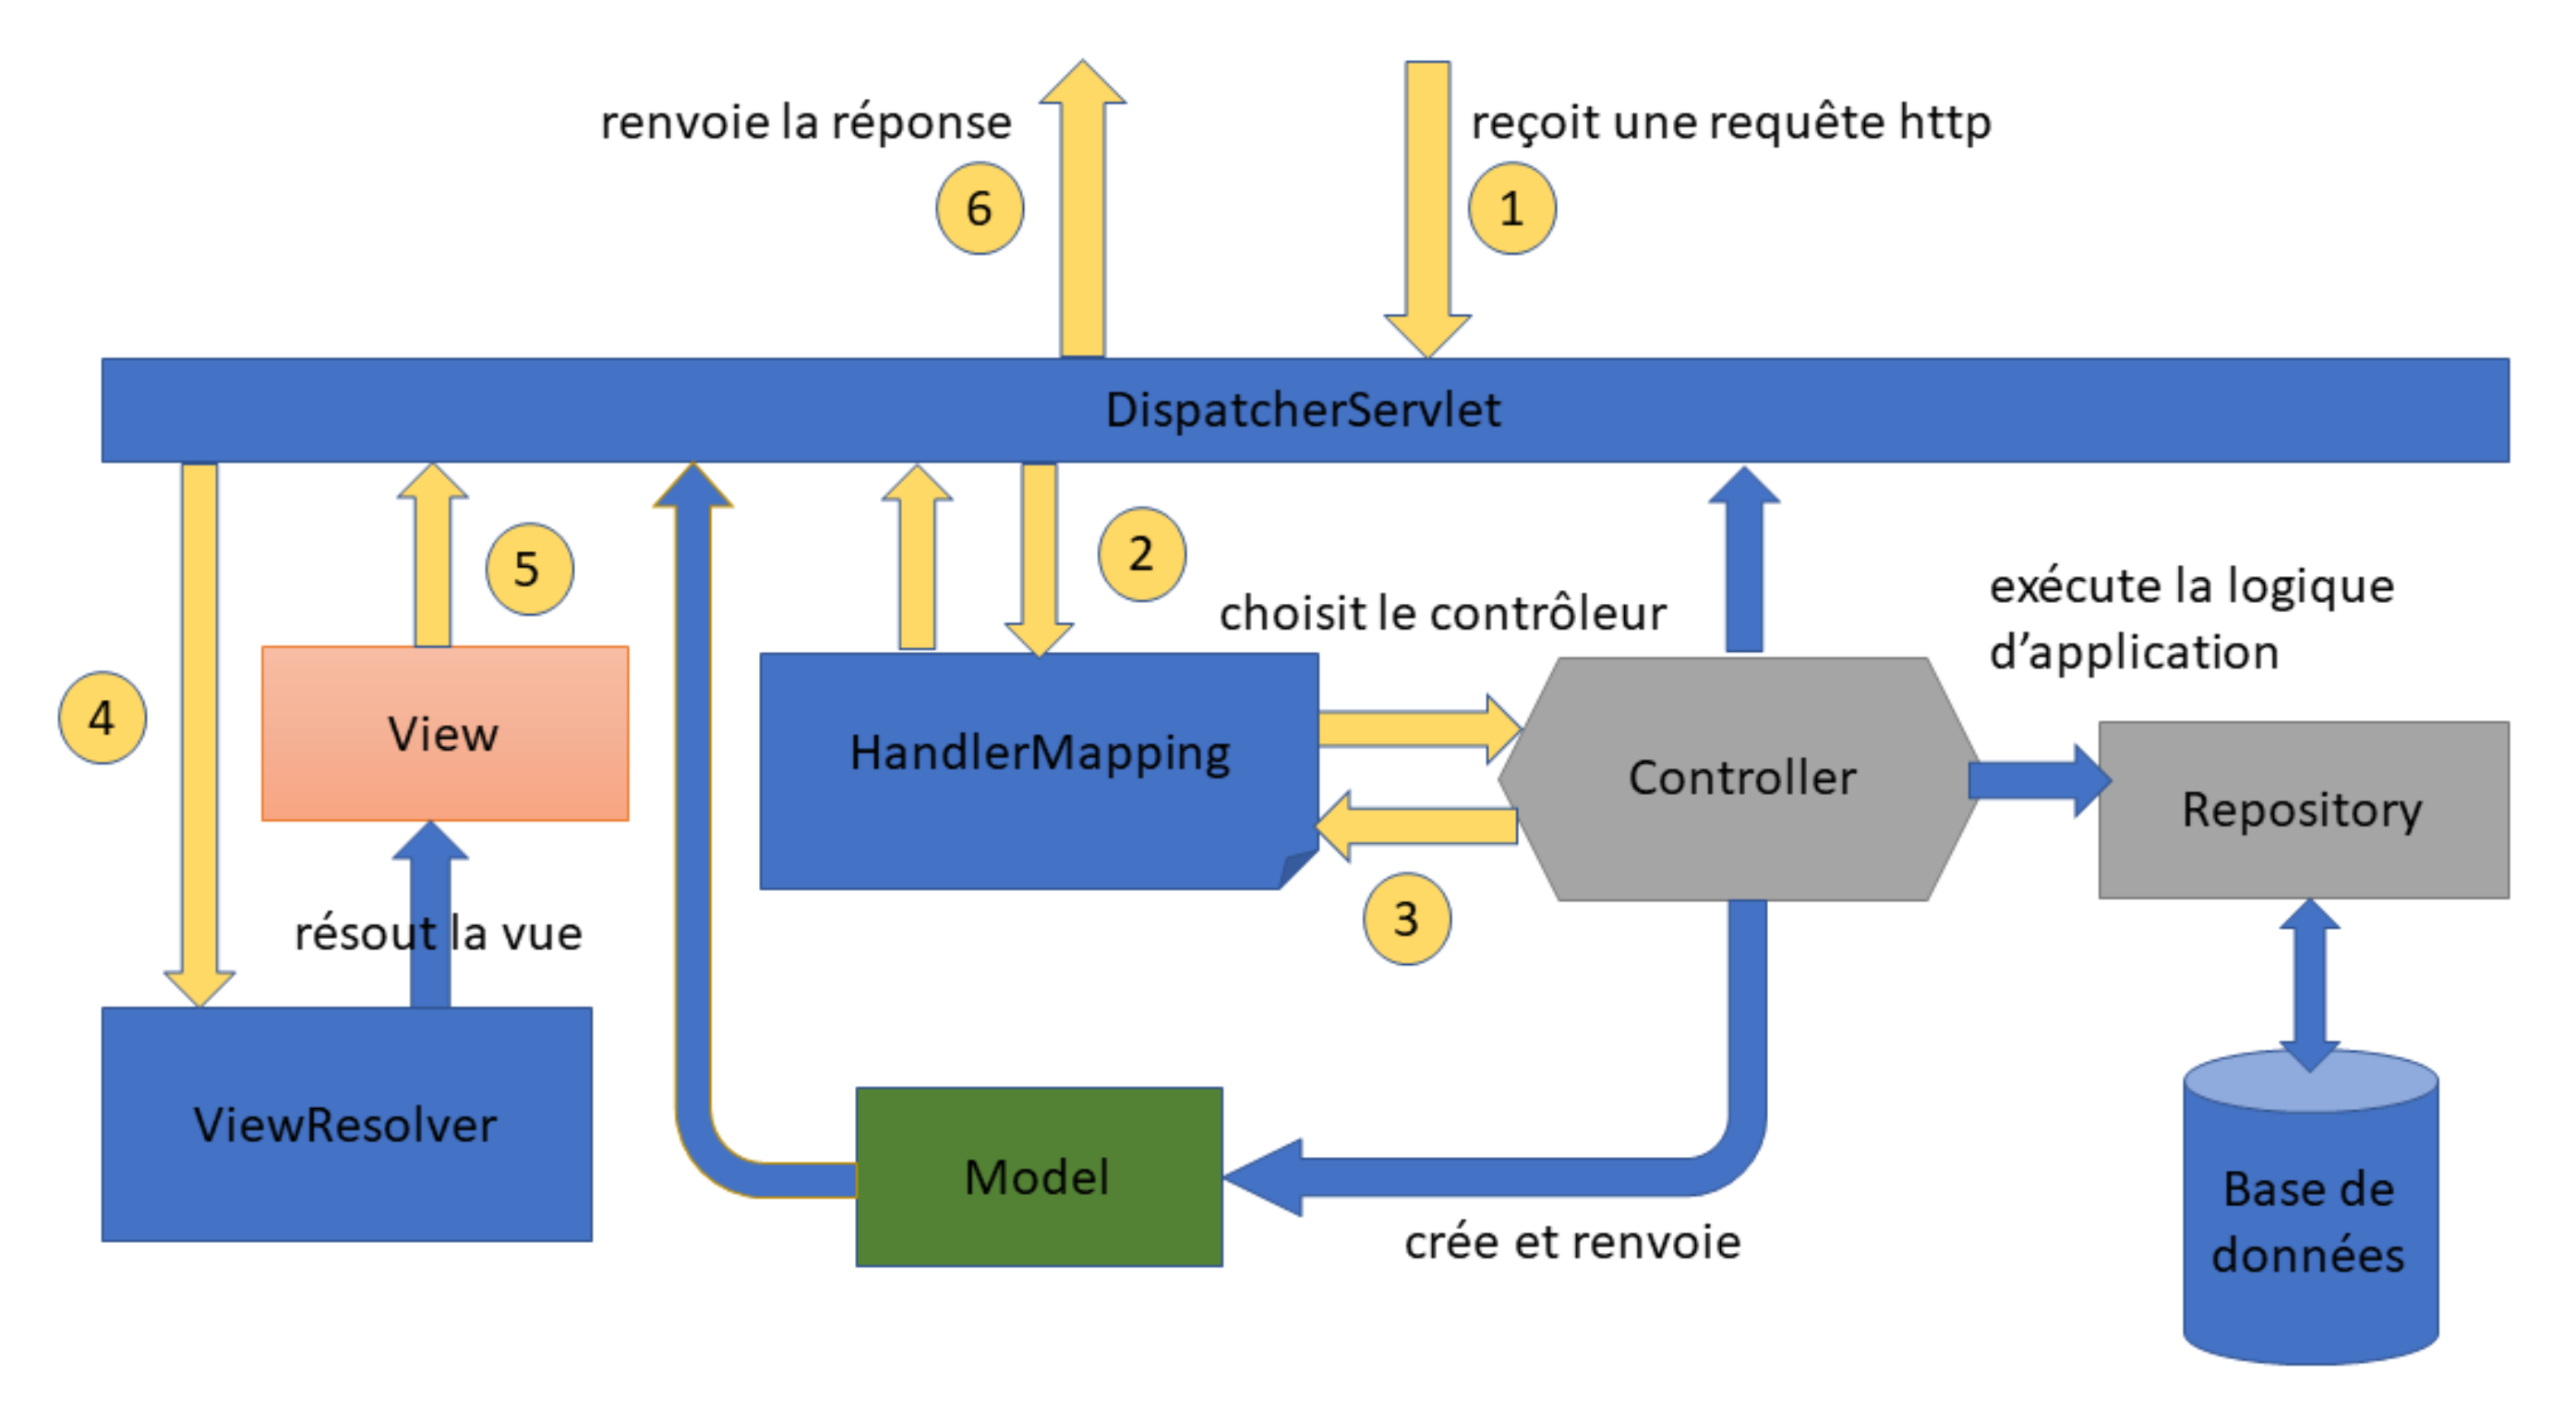
\includegraphics[width=1.0 \columnwidth]{figures/ArchitectureSpring.png}
    \caption{Architecture of the \textit{Spring} framework}
    \label{fig:ArchitectureSpring}
\end{figure}
\end{comment}


\textit{Spring Security} is the library allowing the management of authentication and access control. Like any \textit{Spring} project, it is customizable. 
Authentication being the first security rampart of the application, the issue here is to make sure that this \textit{Authenticator} design pattern is correctly implemented and preserves the desired security properties.
This main motivation has guided our experiment to focus on the application of Security Contracts on the authentication process.

The figure \ref{fig:ArchitectureAuthenticationSpring} details the authentication management within the \textit{Spring} framework. We explain a generic scenario in the figure via the diagram numbers. So when the application developed with \textit{Spring Security} receives a request, a component chain is activated (1) . When the request contains an authentication one, the \textit{AuthenticationFilter} will extract the user's credentials (usually username and password) and create an \textit{Authentication} object. If the received information contains a username and a password, a \textit{UsernamePasswordAuthenticationToken} will be created containing the username and the password (2) . 

This token will be used to invoke the \textit{authenticate()} method of the \textit{AuthenticationManager} which is implemented by \textit{ProviderManager} (3). There are several \textit{AuthenticationProvider} already configured and listed in \textit{ProviderManager}. The one we will use in this experimentation is the \textit{DAOAuthenticationProvider}. DAO stands for "Data Access Object", which is a model that provides an abstract interface to a database type. By mapping application calls to the persistence layer, the DAO provides certain specific data operations without exposing the details of the database. The \textit{DAOAuthenticationProvider} uses \textit{UserDetailsService} (5) to retrieve user data based on the user's username (6) , (7) , (8) , (9). If the authentication (10) succeeds then the complete \textit{Authentication} object (with "authenticated = True", the list of authorities and the user name) is returned. Finally, the \textit{AuthenticationManager} returns the \textit{Authentication} object to the \textit{Authenticationfilter}, the authentication has succeeded and the object is stored in the \textit{SecurityContext}.
And if the authentication fails,  the \textit{AuthenticationManager} raises an exception \textit{AuthenticationException} will be thrown. 

\begin{figure}[!h]
    \centering
    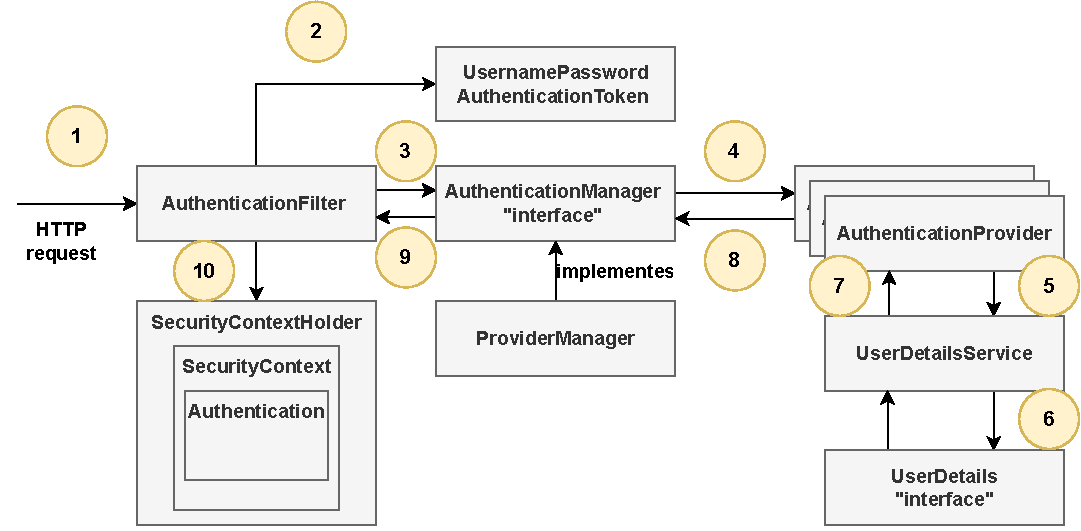
\includegraphics[width=1.0 \columnwidth]{figures/AuthenticateSpringProcess.pdf}
    \caption{Authenticate service in the \textit{Spring} framework}
    \label{fig:ArchitectureAuthenticationSpring}
\end{figure}

\subsection{Applying the \textit{Authenticator} Security Contract on the \textit{Spring} authentication}

% PAMELA: un framework de tissage au run-time permettant de faire du monitoring de propriétés de sécurité

The implementation of the Security Contract \textit{Authenticator} in this context is based on two phases: 1) Weaving the \textit{Authenticator} pattern into the \textit{Spring} architecture, presented just below 2) Allocating the security properties, presented in the section \ref{subsection:secureapplication}, to be preserved by the application.


These two steps are ensured by source code annotation techniques. These techniques are used by the application developer which must know the contract definition, and the application code reused.
First of all, this developer requires the identification of the appropriate concepts and extension points. Sometimes for a reuse perspective inheritance and delegation are used to expand these extension points.

Figure \ref{fig:authclasses} shows the class diagram of the \textit{Authenticator} contract presented in section \ref{subsec:AuthenticatorSecurityContract}. 
%We also refer to figure \ref{fig:AuthenticatorPattern} for the correspondence of the concepts between the business concepts provided by \textit{Spring} and the \textit{Authenticator} contract used.
This contract identifies four distinct entities: \textit{Authenticator}, \textit{Subject}, \textit{AuthenticationInformation} and \textit{ProofOfIdentity}, for which we need to find the corresponding business concept in the source code to be annotated. To examplify our approach, we select only the \textit{Authenticator} and the \textit{Subject} entities.



\subsubsection{Authenticator}: This concept is identified in the \textit{Authenticator} pattern with the \texttt{@Authenticator} annotation. On the application to secure, the Java interface \textit{AuthenticationProvider} plays the corresponding role. So this role is applied, line 3 of the listing \ref{listing:CustomAuthenticationProvider}, to the specialization \textit{CustomAuthenticationProvider} which extends \textit{AuthenticationProvider}. 

From an implementation point of view, the role is implemented by the \textit{CustomAuthenticationProviderImpl} class, presented on line 17 in the listing \ref{listing:CustomAuthenticationProvider}.
This class is extended from \textit{DAOAuthenticationProvider} class which takes care of this role in the Spring framework. 
%To specialize this logic, we use inheritance on the Spring framework API, by defining an API/implementation pair (\textit{DaoAuthenticationProvider} / \textit{CustomAuthenticationProviderImpl}) presented on line 17 in the listing \ref{listing:CustomAuthenticationProvider}. 

The link between the role and the pattern definition is done via the identifier \texttt{SessionInfo.PATTERN_ID}, which is currently a character string, see line 3.


\begin{lstlisting}[language=Java,basicstyle=\ttfamily\footnotesize, caption=Specialization of \textit{Authenticator} entity through \texttt{CustomAuthenticationProvider} definition,label=listing:CustomAuthenticationProvider]
@ModelEntity
@ImplementationClass(CustomAuthenticationProviderImpl.class)
@Authenticator(patternID = SessionInfo.PATTERN_ID)
@Imports(@Import(SessionInfo.class))
public interface CustomAuthenticationProvider extends AuthenticationProvider {
  String USER_NAME = "userName";

  // Inherited from AuthenticationProvider API
  public Authentication authenticate(Authentication authentication) throws AuthenticationException;
    
    ...
    
  abstract class CustomAuthenticationProviderImpl extends DaoAuthenticationProvider implements CustomAuthenticationProvider {

    @Override
    public Authentication authenticate(Authentication authentication) throws AuthenticationException {
      ...
    }

    @Override
    public UsernamePasswordAuthenticationToken request(String userName) {
      ...
    }
  }
}
\end{lstlisting}

\subsubsection{Subject}: 
This concept is identified in the \textit{Authenticator} pattern with the \texttt{@AuthenticatorSubject} annotation, line 3 of the listing \ref{listing:SessionInfo}. On the application to secure, this concept is not directly reified but corresponds to the notion of session, from our point of view. Thus we reify the concept \texttt{SessionInfo}, which is presented in the listing \ref{listing:SessionInfo}. 
The \textit{SessionInfo} concept allows the management of the \texttt{USER_NAME}, \texttt{IP\_ADDRESS} and \texttt{ID\_PROOF} (proof of identity) from line 5 to 10, as well as the access to the authenticator via the accessors \texttt{getAuthenticationProvider()} and \texttt{setAuthenticationProvider()}

The method \texttt{authenticate()} (line 18 of the listing \ref{listing:SessionInfo}) is identified via the annotation \texttt{@AuthenticateMethod} to the method \texttt{request} of the pattern \textit{Authenticator} as presented in the figure \ref{fig:AuthenticatorPattern}.
The \texttt{checkSecure()} method is annotated as \texttt{@RequiresAuthentication}, line 20-21,  to trigger the Authentication process based on the method with the annotation \texttt{@AuthenticateMethod} if the process is executed for the first time. 

\begin{lstlisting}[language=Java,basicstyle=\ttfamily\footnotesize, caption= \texttt{SessionInfo} to implement the \textit{Subject} entity,label=listing:SessionInfo]
@ModelEntity
@ImplementationClass(SessionInfo.SessionInfoImpl.class)
@AuthenticatorSubject(patternID = SessionInfo.PATTERN_ID)
public interface SessionInfo {

	String SESSION_INFO = "SESSION_INFO";
	String PATTERN_ID = "AuthenticatorPattern";
	String USER_NAME = "username";
	String IP_ADRESS = "ipAdress";
	String AUTHENTICATION_PROVIDER = "authenticationProvider";
	String ID_PROOF = "idProof";

    ....
    
	@Getter(AUTHENTICATION_PROVIDER)
	@AuthenticatorGetter(patternID = PATTERN_ID)
	CustomAuthenticationProvider getAuthenticationProvider();

	@Setter(AUTHENTICATION_PROVIDER)
	void setAuthenticationProvider(CustomAuthenticationProvider val);

    ....
    
	@AuthenticateMethod(patternID = PATTERN_ID)
	void authenticate();

	@RequiresAuthentication
	void checkSecure();

	abstract class SessionInfoImpl implements SessionInfo {

        ...
        
		@Override
		public void checkSecure() {
			System.out.println("checkSecure() for " + this);
		}

		@Override
		public String getIpAdress() {
			return ((ServletRequestAttributes)RequestContextHolder.currentRequestAttributes())
			           .getRequest().getRemoteAddr();
		}
	}

}
\end{lstlisting}

\begin{comment}

\subsubsection{AuthenticationInformation}: The information at the base of the authentication in the \textit{Spring} application to be secured is the user name defined in the \textit{SessionInfo} class (listing \ref{listing:SessionInfo}). A character string implements the user name and its accessed by \texttt{getUserName()} and \texttt{setUserName(String)} defined respectively lines 15 and 18 of the listing \ref{listing:SessionInfo}. The annotation \texttt{@AuthenticationInformation} defined on line 14 specifies the use of this data for authentication, together with the annotation \texttt{@AuthenticationInformation(paramId=...)} defined on line 14 of the listing \ref{listing:CustomAuthenticationProvider}.

\subsubsection{ProofOfIdentity}: The fourth and last entity to be identified is the notion of proof of identity which is found in the \texttt{UsernamePasswordAuthenticationToken} class in the \textit{Spring} application. We have chosen to expose the accessors getIDProof() and setIDProof(UsernamePasswordAuthenticationToken) in the SessionInfo interface (respectively lines 27 and 31 of the listing \ref{listing:SessionInfo}.


\subsubsection{Life cycle of the \texttt{AuthenticationProvider} concept}:
We have used the notion of \textit{Service} offered by the \textit{Spring} framework to implement a service dedicated to authentication. The listing \ref{listing:AuthManagerService} presents this implementation. This service is responsible to instantiate a single instance (singleton design pattern) of \texttt{CustomAuthenticationProvider} for the application. As well, this service creates a session with an instance of (\texttt{SessionInfo}), via the use of a factory based on the construction of the \texttt{PamelaMetaModel} inferred from the \texttt{CustomAuthenticationProvider} class (lines 11 and 12 of the listing \ref{listing:AuthManagerService}). 


\begin{lstlisting}[language=Java,basicstyle=\ttfamily\footnotesize, caption=Mise en oeuvre du service d'authentification : \texttt{AuthManagerService.java},label=listing:AuthManagerService]
@Service
public class AuthManagerService {

	private CustomAuthenticationProvider authenticationProvider;

	private PamelaModelFactory factory;

	public AuthManagerService() {
		PamelaMetaModel pamelaMetaModel;
		try {
			pamelaMetaModel = new PamelaMetaModel(CustomAuthenticationProvider.class);
			factory = new PamelaModelFactory(pamelaMetaModel);
		} catch (ModelDefinitionException e) {
			e.printStackTrace();
		}

		authenticationProvider = factory.newInstance(CustomAuthenticationProvider.class);
	}

	public CustomAuthenticationProvider getAuthenticationProvider() {
		return authenticationProvider;
	}

	public SessionInfo makeNewSessionInfo() {
		SessionInfo returned = factory.newInstance(SessionInfo.class);
		returned.setAuthenticationProvider(getAuthenticationProvider());
		return returned;
	}
}
\end{lstlisting}

\subsubsection{Lifecycle of the session concept by the \texttt{SessionInfo}}: 
We used the \textit{Spring} component \texttt{HttpSessionEventPublisher} as a support for extension points allowing to manage the construction and destruction of instances of \texttt{SessionInfo}. We propose in the listing \ref{listing:CustomHttpSessionEventPublisher} a class \texttt{CustomHttpSessionEventPublisher} which inherits from \texttt{HttpSessionEventPublisher} and which implements these functionalities of management of instances of \texttt{SessionInfo} (lines 12 and 21 respectively for the creation and the destruction of instances).


\begin{lstlisting}[language=Java,basicstyle=\ttfamily\footnotesize, caption=Cycle de vie des \texttt{SessionInfo} : \texttt{CustomHttpSessionEventPublisher.java},label=listing:CustomHttpSessionEventPublisher]
@Component
public class CustomHttpSessionEventPublisher 
extends HttpSessionEventPublisher {

	@Autowired
	private AuthManagerService authManagerService;

	@Override
	public void sessionCreated(HttpSessionEvent event) {
		super.sessionCreated(event);
		if (event.getSession().getAttribute(SessionInfo.SESSION_INFO) == null) {
			SessionInfo sessionInfo = authManagerService.makeNewSessionInfo();
			event.getSession().setAttribute(SessionInfo.SESSION_INFO, sessionInfo);
		}
	}

	@Override
	public void sessionDestroyed(HttpSessionEvent event) {
		super.sessionDestroyed(event);
		// delete the session
    ((SessionInfo)event.getSession().getAttribute(SessionInfo.SESSION_INFO)).delete();
	}
}
\end{lstlisting}
\end{comment}


\subsubsection{Authentication management}: 
The management of authentication itself is intricate because of two competing levels: the authentication provided by the \textit{Spring} framework and the one implemented in our \textit{Authenticator} pattern. The alignment of the two mechanisms takes place in the implementation of \texttt{CustomAuthenticationProviderImpl} (listing \ref{listing:CustomAuthenticationProviderImpl}). The \textit{Spring} framework receives the authentication requests via the call of the method \texttt{authenticate(Authentication)} of \texttt{AuthenticationProvider}. We overwrite this method, line 13,  with the management of the current session information (from line 16 to 23), and the  \texttt{authenticate()} and  \texttt{checkSecure()} of the  \texttt{SessionInfo} entity, line 24 to 27, are called to complete the process.
%but especially by filling a table of correspondence between the username used as authentication information and the proof of identity returned by the \texttt{AuthenticationProvider} (an instance of \texttt{UsernamePasswordAuthenticationToken}). The implementation of the \texttt{request(String)} method is limited to returning this same value.

\begin{lstlisting}[language=Java,basicstyle=\ttfamily\footnotesize, caption=Authentication management with \texttt{CustomAuthenticationProvider} definition,label=listing:CustomAuthenticationProviderImpl]
abstract class CustomAuthenticationProviderImpl extends DaoAuthenticationProvider implements CustomAuthenticationProvider {

    private Map<String, UsernamePasswordAuthenticationToken> tokens 
        = new HashMap<>();
        
	/**
      * Implementation is here trivial as we use map filled by
      * {@link #authenticate(Authentication)} method
		 */
	@Override
	public UsernamePasswordAuthenticationToken request(String userName) {
		return tokens.get(userName);
	}

	@Override
	public Authentication authenticate(Authentication authentication) throws AuthenticationException {

		try {
			System.out.println("authenticate(Authentication) called for " + authentication);
			UsernamePasswordAuthenticationToken returned = (UsernamePasswordAuthenticationToken) super.authenticate(authentication);
			String name = authentication.getName();
			WebAuthenticationDetails details = (WebAuthenticationDetails) authentication.getDetails();
			String userIp = details.getRemoteAddress();
			SessionInfo sessionInfo = SessionInfo.getCurrentSessionInfo();
			sessionInfo.setUserName(name);
			sessionInfo.setIpAdress(userIp);
			tokens.put(name, returned);
			// Call authenticate() to complete process
			sessionInfo.authenticate();
			// Ensure that we are now in authenticated context
			sessionInfo.checkSecure();
			return returned;
		} catch (AuthenticationException e) {
			throw e;
		} catch (ModelExecutionException e) {
			e.printStackTrace();
			throw new SessionAuthenticationException("Exception during authentication: " + e.getMessage());
        }

	}
}
\end{lstlisting}


\subsection{Pattern \textit{Authenticator} specialisation to extend the behavior with a temporal logic property}


% discours sur ok on a définit le contrat et maintenant on étend avec une nouvelle prop et on customize la classe du framework.




One of the interests of our approach lies in the ability of the framework to provide extension points. In our case, the \texttt{CustomAuthenticationProvider} class specializes our implementation of the \textit{Authenticator} pattern.
            

 The second feature of our framework that we exploit, is the reification of the notion of instance of the \textit{Authenticator} pattern through the instance of the \texttt{AuthenticatorPatternInstance} class, see figure \ref{fig:AuthenticatorPattern}. 
This class encapsulates the instances of the subject (class \texttt{SessionInfo}) and authenticator (class \texttt{CustomAuthenticationProvider}). 
%L'exécution de ces classes est tissée au run-time. 
%The execution of these classes is woven into the run-time. 
As this class gives access to the instances of the classes of the pattern, an introspection capacity of the current state of the pattern is provided during all its life cycle. 
% et donc de l'exécution de code métier lié à l'assemblage de ces classes.

We have taken advantage of these two aspects to specialize the \textit{Authenticator} pattern by extending the behavior with a new temporized temporal property. This property takes into account a time quantity applied on an execution path of the pattern. Classically this property expresses the fact that there cannot be more than three authentication failures in a given period of time. If three failures occur in this time, the application will have to switch to another mode, classically refusing any authentication attempt for a certain time for example.

Let $auth\_fail_i$ be an "authentication failure" event in the current execution trace:

    \begin{equation*}
       \begin{split}
           P7:& \forall \{ auth\_fail_i,auth\_fail_{i+1},auth\_fail_{i+2} \} \in execution\_trace \\
          &auth\_fail_{i+2}.time - auth\_fail_i.time < TIME\_LIMIT
      \end{split}
    \end{equation*}


The class \texttt{CustomAuthenticatorPatternInstance}, listing  \ref{listing:CustomAuthenticatorPatternInstance}, implements the definition of the property \textit{P7} through the method \texttt{checkRecentAuthFailCountLessThan3} from lines 7 to 15.
This property is based on the evaluation of the \texttt{events} variable, defined line 3, which is defined as an instance variable of this class.  This variable \texttt{events} embodies the current state of the class's instances and takes part of the global state of the pattern. 
%This pattern state consists of the internal state of each class instance of the pattern. 
In our example, this variable is updated, line 17, to take into account each authentication failure and so assessed for the property evaluation.    

After the definition of the contract property, the listing \ref{listing:TemporalPropertyDefinition} presents the definition of the \textit{Authenticator} referring to this property as a precondition of the method \texttt{authenticate()} (line 9). Also we can see between the line 4 and 8, the use of the annotation \texttt{@OnException} which allows to automatically generate events corresponding to the failure of connection. This events is stored in the pattern state via the \texttt{events} variable as we described before.

%first the three listing classes \ref{listing:CustomAuthenticatorPatternFactory}, \ref{listing:CustomAuthenticatorPatternDefinition} and \ref{listing:CustomAuthenticatorPatternInstance}. 




\begin{comment}
\begin{lstlisting}[language=Java,basicstyle=\ttfamily\footnotesize, caption=Spécialisation de la classe \texttt{AuthenticatorPatternFactory.java},label=listing:CustomAuthenticatorPatternFactory]
public class CustomAuthenticatorPatternFactory extends AuthenticatorPatternFactory {

	public CustomAuthenticatorPatternFactory(PamelaMetaModel metaModel) {
		super(metaModel);
	}

	@Override
	protected Class<CustomAuthenticatorPatternDefinition> getPatternDefinitionClass() {
		return CustomAuthenticatorPatternDefinition.class;
	}

	@Override
	protected CustomAuthenticatorPatternDefinition getPatternDefinition(String patternId, boolean createWhenNonExistant) {
		return (CustomAuthenticatorPatternDefinition) super.getPatternDefinition(patternId, createWhenNonExistant);
	}
}
\end{lstlisting}




\begin{lstlisting}[language=Java,basicstyle=\ttfamily\footnotesize, caption=\texttt{CustomAuthenticatorPatternDefinition} specializes \texttt{AuthenticatorPatternDefinition},label=listing:CustomAuthenticatorPatternDefinition]
public class CustomAuthenticatorPatternDefinition extends AuthenticatorPatternDefinition {

	public CustomAuthenticatorPatternDefinition(String identifier, PamelaMetaModel pamelaMetaModel) {
		super(identifier, pamelaMetaModel);
	}

	@Override
	public <I> void notifiedNewInstance(I newInstance, ModelEntity<I> modelEntity, PamelaModel model) {
		if (modelEntity == getSubjectModelEntity()) {
			// We create a new PatternInstance for each new instance of subjectModelEntity
			CustomAuthenticatorPatternInstance<?, I, ?, ?> newPatternInstance = new CustomAuthenticatorPatternInstance(this, model,
					newInstance);
		}
	}
}
\end{lstlisting}

\end{comment}



\begin{lstlisting}[language=Java,basicstyle=\ttfamily\footnotesize, caption=\texttt{AuthenticatorPatternInstance} specialization to add the P7 property implementation,label=listing:CustomAuthenticatorPatternInstance]
public class CustomAuthenticatorPatternInstance extends AuthenticatorPatternInstance<CustomAuthenticationProvider, SessionInfo, String, UsernamePasswordAuthenticationToken> {

	public static long TIME_LIMIT = 180000; // 180s = 3 min

	private List<PatternInstanceEvent> events = new ArrayList<>();

	public CustomAuthenticatorPatternInstance(CustomAuthenticatorPatternDefinition patternDefinition, PamelaModel model, SessionInfo subject) {
		super(patternDefinition, model, subject);
	}

	// Perform check that last 3 AuthFailEvent in current execution trace were not raised within allowed time limit
	public boolean checkRecentAuthFailCountLessThan3() {
		long currentTime = System.currentTimeMillis();
		if (events.size() >= 3 && (currentTime - events.get(events.size() - 3).getDate()) < TIME_LIMIT) {
			// 3 attempts or more in TIME_LIMIT interval
			return false;
		}
		return true;
	}

	public void generateAuthFailEvent() {
			events.add(new AuthFailedEvent());
    }

	@Override
	public void authenticationSuceeded() {
		super.authenticationSuceeded();
	}
 }
\end{lstlisting}


The extension of the previous contract being realized, we can now use it and add an \texttt{@ensures} annotation with a reference to the implementation of the new property, line 9 of the listing \ref{listing:TemporalPropertyDefinition}.
This annotation is defined related to the \texttt{authenticate()} method.
So for now, any call of this method respects the security contract defined by the instance \texttt{CustomAuthenticatorPatternInstance} corresponding to the current execution. This contract automatically handles the \texttt{AuthFailedEvent} events, and checks that a user cannot fail to authenticate more than 3 times in a given time. 




\begin{lstlisting}[language=Java,basicstyle=\ttfamily\footnotesize, caption=Contract definition with applying with the P7 property,label=listing:TemporalPropertyDefinition]
public interface CustomAuthenticationProvider extends AuthenticationProvider {

    ...
    
	@Override
	@OnException(
			patternID = SessionInfo.PATTERN_ID,
			onException = AuthenticationException.class,
			perform = "patternInstance.generateAuthFailEvent()",
			strategy = OnExceptionStategy.HandleAndRethrowException)
	@Ensures(patternID = SessionInfo.PATTERN_ID, property = "patternInstance.checkRecentAuthFailCountLessThan3()")
    public Authentication authenticate(Authentication authentication) throws AuthenticationException;

    ...
}
\end{lstlisting}


Our use case shows how to extend the \textit{Authentication} process, based on an existing code, to ensure a security contract that verifies the properties P1-P7 defined at design time. Note that the full code of this case study can be found at the web site of the project~\footnote{https://github.com/openflexo-team/pamela/tree/2.0/pamela-spring-security-uc}.

With this experiment, we sought to demonstrate:
\begin{itemize}
    \item the definition of a security contract allows us to highlight the properties we seek to preserve, independently of the implementation.
    \item this definition allows to increase the level of abstraction of the classical definition of security patterns, even on a conceptual class diagram.
    \item these contracts allow the link between the Security by Design and Execution under Contract phases, which remains a problem not enough covered at present, without code generation.
    \item The use case treated also shows that the weaving of a security contract by specialization of an existing pattern, is possible and easily usable based on code annotation.
    \item the specialization of the security contract can also be progressive by extending the number of properties and specializing the code defining the contract. 
\end{itemize}

